


\newpage
\appendix
%\begin{center}

% {\huge \textbf{Appendix \\ Achieving robustness in classification using optimal transport with hinge regularization}}
% \end{center}
\section{Optimal transportation : discrete case}
\subsection{Optimal transport}
\label{secOptTransp}
When considering a limited number of samples for the two distribution, the computation of the Wasserstein distance 
%is an optimal transportation problem that 
can be solved through linear programming algorithms. In the balanced case, we have $X=\{x_1, \ldots, x_{2n}\}$ where $\{x_1,\ldots,x_n\}$ are sampled from $P_+$ and  $\{x_{n+1},\ldots,x_{2n}\}$ are sampled from $P_-$. We note $U=\{u_1, \ldots, u_{2n}\}$ the labels with $u_1,\ldots,u_n=1$ and $u_{n+1},\ldots,u_{2n}=-1$ and $C$ the $n\times n$ matrix cost function with $C_{i,j}=||x_i-x_{n+j}||$. The primal problem of the optimal transport is to find a transportation plan $\Pi$ (a $n\times n$ matrix) such as:
\begin{alignat}{2}
&\!\min_{\Pi}        &\qquad& \sum_{i,j \in n\times n}\Pi_{i,j}*C_{i,j}\\
&\text{subject to} &      & \Pi_{i,j} \geq 0,\\
&                  &      & \sum_i \Pi_{i,j} = \frac{1}{n},\sum_j \Pi_{i,j} = \frac{1}{n}.
\end{alignat}
The constraints enforce $\Pi$ to be a discrete joint probability distribution with the appropriate marginals as in the continuous case. The dual formulation for the discrete optimal transport problem is:
\begin{alignat}{2}
&\!\max_{F}        &\qquad& F.U^T\\
&\text{subject to} &      & \forall i,j \in n\times n, F_i-F_{n+j}\leq C_{i,j}
\end{alignat}
where $F$ is a $2n$ vector that is a discrete version of the function $f$ of Equation \ref{kantorovich}. The constraint on $F$ is the discrete counterpart of the 1-Lipschitz constraint. 

\subsection{Hinge regularized Optimal transport}
Similarly to the classical case, the discrete counterpart of the regularized Wasserstein distance is also a transportation problem which has the following formulation:
\begin{alignat*}{2}
&\!\min_{\Pi}        &\qquad& \sum_{i,j \in n\times n}\left[\Pi_{i,j}*C_{i,j}\right]-2\left(1-\sum_{i,j \in  n\times n}\left[\Pi_{i,j}\right]\right)\\
&\text{subject to} &      & \Pi_{i,j} \geq 0,\\
&                  &      & \frac{1}{n} \leq \sum_i \Pi_{i,j} \leq  \frac{1+\lambda}{n},\\
&                  &      & \frac{1}{n} \leq \sum_j \Pi_{i,j} \leq  \frac{1+\lambda}{n}.
\end{alignat*}
Roughly speaking, it allows to give more weight to the transportation of the closest pairs by admitting to deviate from the marginals with a tolerance that depends on $\lambda$. Since the closest pairs in the two distributions are the most difficult to classify, it illustrates why this formulation is more adequate for classification problem. 
The dual formulation of this transportation problem is a discrete counterpart of Equation \ref{eq:reg_OT} :
\begin{alignat*}{2}
&\!\max_{F}        &\qquad& \sum_{k =0}^{2n} \left[F_i*u_i -\lambda (0,1-F_i*u_i)_+\right]\\
&\text{subject to} &      & \forall i,j \in n\times n, F_i-F_{n+j}\leq C_{i,j}.
\end{alignat*}
We observe that the constraint in the dual problem are not affected by the new formulation and still corresponds to a the 1-Lipschitz constraint in the continuous case. 


\section{Theorem proofs}
\label{appendix:proofs}
\subsection{Proof Theorem 1}
We denote as 
\begin{align}\label{eq:defwoth}
	f^*:=f_{\lambda}^*\in{\arg\min}_{f\in \text{Lip}_1(\Omega)}\mathcal{L}^{hKR}_\lambda(f)\ \ \text{and} \ \ \hat{f}_n:=\hat{f}_{n,\lambda}\in{\arg\min}_{f\in \text{Lip}_1(\Omega)}\hat{\mathcal{L}}^{hKR}_{\lambda,n}(f).
\end{align}
If we assume that \eqref{eq:M} is not true, then there exists $\textbf{x}\in \Omega$ such that $f^*(\textbf{x})>1+\text{diam}(\Omega)+\frac{\mathcal{R}(\psi)}{\inf(p,1-p)}$ or $f^*(\textbf{x})<-1-\text{diam}(\Omega)-\frac{L_1(\psi)}{\inf(p,1-p)}$. We suppose without loss of generality that the first inequality holds. If ${{\textbf{z}}}\in \Omega $ then the 1-Lipschitz condition in $f^*$ implies that $f^*({{\textbf{z}}})>1+\frac{L_1(\psi)}{1-p}$. Hence $(1-f^*)_+=0$ and
\begin{align*}
	L(f^*)&\leq \sup_{g\in Lip_1(\Omega)} L_2(g)- \lambda L_1(f^*)\\
	&=\sup_{g\in Lip_1(\Omega)}E_{X|Y=1}(g(X))-E_{X|Y=-1}(g(X))-E\left\{\lambda (1-Yf^*(X))_+\right\}\\
	&= L_2(\psi)-\lambda \{ pE_{X|Y=1}(1-f^*(X))_++(1-p)E_{X|Y=-1}(1+f^*(X))_+\}\\
	&\leq L_2(\psi)-\lambda \{ (1-p)E_{X|Y=-1}(1+f^*(X))\}\\
	&\leq  L_2(\psi)-\lambda \{ (1-p)E_{X|Y=-1}(2+\frac{L_1(\psi)}{1-p})\} \\
	&= L_2(\psi)-2\lambda(1-p) -\lambda \{ E_{X|Y=-1}({L_1(\psi)})\}=L_2(\psi)-2\lambda(1-p)-\lambda L_1(\psi) 
\end{align*}
Then $f^*$ can not be an optimal solution of the problem \eqref{eq:defwoth}. Then there exists some constant $M$ large enough, such that $f^*$ belongs to $\text{Lip}^M_1(\Omega):=\{f\in \text{Lip}_1(\Omega): || f||_{\infty}\leq M\}$ and not to $\text{Lip}_1(\Omega)$. Since the functional $\mathcal{L}^{hKR}_\lambda$ is convex and $\text{Lip}^M_1(\Omega)$ is compact in $\mathcal{C}(\Omega)$, we are able to make use of Ascoli-Arzela Theorem and conclude that there exists at least one function minimizing the expected loss. Furthermore the set of those functions is compact and convex.


\subsection{Proof Theorem 2}
\begin{Definition}
Let $\mu, \nu$ two positive measures in $\R^d$. The Kullback-Leibler divergence from $\mu$ to $\nu$ is defined as 
\begin{align}
KL(\mu |\nu )=\begin{cases} 
      \int \log(\frac{d\mu}{d\nu})d\mu-\int d\mu+\int d\nu & \text{if} \ \ \mu  << \nu\\
      \infty & otherwise 
   \end{cases}
\end{align}
\end{Definition}
\begin{Theorem}\label{Theo:generaldual}
Let $\phi_1, \phi_2:\Omega\rightarrow \bar{\R}$ be lower semicontinuous convex functions and $\mu, \nu\in \mathcal{P}(\Omega)$ be probability measures. Then for all $\epsilon>0$ the following equality holds
\begin{align}\label{eq:dual_app}
\begin{split}
	&\inf_{\pi \in\Pi_+(\mu, \nu)} \int{\phi_1(-\frac{d\pi_\textbf{x}}{d\mu}(\textbf{x}))d\mu}(\textbf{x})+\int{\phi_2(-\frac{d\pi_{{\textbf{z}}}}{d\nu}({{\textbf{z}}}))d\nu}({{\textbf{z}}})+\epsilon KL(\pi|e^{-\frac{c(\textbf{x},{{\textbf{z}}})}{\epsilon}}(d\mu\times d\nu))\\&= \sup_{f,g\in L^1(\Omega)}-\int_{\Omega}\phi_1^*(f(\textbf{x}))d\mu(\textbf{x})-\int_{\Omega}\phi_1^*(g({{\textbf{z}}}))d\nu({{\textbf{z}}})-\epsilon \int \left(e^{\frac{f(\textbf{x})+g({{\textbf{z}}})-c(\textbf{x},{{\textbf{z}}})}{\epsilon}}-e^{-\frac{c(\textbf{x},{{\textbf{z}}})}{\epsilon}}\right)d\mu d\nu.
	\end{split}
\end{align}
Furthermore if $\epsilon=0$ then
\begin{align}\label{eq:dual_app_zero}
\begin{split}
	&\inf_{\pi \in\Pi_+(\mu, \nu)}\int_{\Omega\times \Omega}c(\textbf{x},{{\textbf{z}}})d\pi(\textbf{x},{{\textbf{z}}}) + \int{\phi_1(-\frac{d\pi_\textbf{x}}{d\mu}(\textbf{x}))d\mu}(\textbf{x})+\int{\phi_2(-\frac{d\pi_{{\textbf{z}}}}{d\nu}({{\textbf{z}}}))d\nu}({{\textbf{z}}})\\&= \sup_{(f,g)\in \Phi(\mu, \nu)}-\int_{\Omega}\phi_1^*(f(\textbf{x}))d\mu(\textbf{x})-\int_{\Omega}\phi_1^*(g({{\textbf{z}}}))d\nu({{\textbf{z}}}).
	\end{split}
\end{align}
Where $\Pi_+(\mu, \nu)$ is the set of positive measures $\pi\in \mathcal{M}_+(\Omega\times \Omega)$ which are absolutely continuous  with respect to the joint measure $d\mu\times d\nu$, and $\Phi(\mu, \nu)$ consists of the pairs of functions $(f,g)\in L_1(\Omega)\times L_1(\Omega)$ such that $c(\textbf{x},{{\textbf{z}}})-f(\textbf{x})-g({{\textbf{z}}}) \geq 0$ $ d\mu\times d\nu -a.s.$.
\end{Theorem}

First we recall the Fenchel–Rockafellar Duality result, we use a weaker version given in Theorem 1.12 in \cite{Brez}
\begin{Proposition} \label{Fenchel–Rockafellar}
Let $E$ be a Banach space and $\Upsilon,\Psi:E\rightarrow \R \cup \{\infty \}$ be two convex functions, assume that there exist ${{\textbf{z}}}_0\in\text{dom}(\Psi)\cap \text{dom}(\Upsilon) $ such that $\Psi$ is continous in ${{\textbf{z}}}_0$. Then strong duality holds
\begin{align} \label{FC}
\inf_{a\in E}\left\lbrace \Upsilon(a)+\Psi(a)\right\rbrace=\sup_{b\in E^*}\left\lbrace -\Upsilon^*(-b)-\Psi^*(b)\right\rbrace
\end{align}
\end{Proposition} 
We identify the different elements of our problem with such of previous Proposition. 
\begin{itemize}
\item $E$ is the space of continuous functions in $\Omega\times \Omega$. Note that the set is bounded, hence $E^*$, by Riesz theorem, is the set of regular measures in $\Omega\times \Omega$.
\item If $\epsilon=0:$
\begin{align}
\Psi_0(u)&=\begin{cases} 
      0 & \text{if} \ \ u(\textbf{x},{{\textbf{z}}})\geq -c(\textbf{x},{\textbf{z}})\\
      \infty & \text{otherwise }
   \end{cases}\\ 
\Upsilon_0(u)&= \begin{cases} 
      \int \phi_1^*(-f(\textbf{x}))d\mu(\textbf{x})+\int \phi_2^*(-g({{\textbf{z}}})) d\nu({{\textbf{z}}})  & \text{if} \ \ u(\textbf{x},{\textbf{z}})=f(\textbf{x})+g({\textbf{z}})\\ 
      \infty & \text{otherwise } 
   \end{cases}
\end{align}
If $\epsilon>0$:
\begin{align}
\Psi_{\epsilon}(u)&=\epsilon \int \left(e^{\frac{u(\textbf{x},{{\textbf{z}}})-c(\textbf{x},{\textbf{z}})}{\epsilon}}-e^{-\frac{c(\textbf{x},{\textbf{z}})}{\epsilon}}\right)d\mu(\textbf{x}) d\nu({{\textbf{z}}})\\ 
 \Upsilon_{\epsilon}(u)&=\Upsilon_0(u)
\end{align}
\end{itemize}
Note that $ \Upsilon_{\epsilon}(u)=\Upsilon_0(u)$ could be non well defined, to avoid this situation we fix $\textbf{x}_0\in \Omega$ and consider $u(\textbf{x},{{\textbf{z}}})=(u(\textbf{x},{{\textbf{z}}}_0)-u({{\textbf{z}}}_0,{{\textbf{z}}}_0)/2)+u({{\textbf{z}}}_0,{{\textbf{z}}})-u({{\textbf{z}}}_0,{{\textbf{z}}}_0)/2)$. 
Now we compute the dual operators 
\begin{align*}
\Psi^*_{\epsilon}(-\pi)&=\sup_{u\in E}\left\lbrace  -\epsilon\int \left(e^{\frac{u(\textbf{x},{{\textbf{z}}})-c(\textbf{x},{\textbf{z}})}{\epsilon}}-e^{-\frac{c(\textbf{x},{\textbf{z}})}{\epsilon}}\right)d\mu(\textbf{x}) d\nu({{\textbf{z}}})-\int u(\textbf{x},{\textbf{z}})d\pi(\textbf{x},{{\textbf{z}}}) \right\rbrace\\
&=\sup_{u\in E}\left\lbrace -\epsilon\int \left(e^{\frac{u(\textbf{x},{\textbf{z}})-c(\textbf{x},{{\textbf{z}}})}{\epsilon}}-e^{-\frac{c(\textbf{x},{{\textbf{z}}})}{\epsilon}}\right)d\mu(\textbf{x}) d\nu({{\textbf{z}}})+\int u(\textbf{x},{{\textbf{z}}})d\pi(\textbf{x},{{\textbf{z}}}) \right\rbrace
\end{align*}
Now if $\pi$ were not absolutely continuous respect the joint measure $e^{-\frac{c(\textbf{x},{{\textbf{z}}})}{\epsilon}}d\mu\times d\nu$ then we would have a continuous function $u(\textbf{x},{{\textbf{z}}})=0$ $d\mu\times d\nu$ almost surely and such that $\int u(\textbf{x},{{\textbf{z}}})d\pi(\textbf{x},{{\textbf{z}}})\neq 0$. If we take the function $\lambda u({{\textbf{z}}},{{\textbf{z}}})$ and $\lambda$ tends to $\pm \infty$ we deduce that the supremum is $\infty $. Then suppose that $d\pi =m(\textbf{x},{{\textbf{z}}})e^{-\frac{c(\textbf{x},{{\textbf{z}}})}{\epsilon}}(d\mu\times d\nu)$.
\begin{align*}
\Psi^*_{\epsilon}(-\pi)&= \begin{cases} 
      \sup_{u\in E}\left\lbrace \epsilon\int \left(-e^{\frac{u(\textbf{x},{{\textbf{z}}})}{\epsilon}}+1 +\frac{u(\textbf{x},{{\textbf{z}}})}{\epsilon}m(\textbf{x},{{\textbf{z}}})\right) e^{-\frac{c(\textbf{x},{{\textbf{z}}})}{\epsilon}}d\mu(\textbf{x}) d\nu({{\textbf{z}}}) \right\rbrace & \text{if $d\pi =m e^{-\frac{c(\textbf{x},{{\textbf{z}}})}{\epsilon}}(d\mu\times d\nu)$.} \\
      \infty & \text{otherwise. } 
   \end{cases}\\
   &=  \epsilon KL(\pi|e^{-\frac{c(\textbf{x},{{\textbf{z}}})}{\epsilon}}(d\mu\times d\nu) ) & 
\end{align*}
With some similar calculation, we compute for $\epsilon=0$:
\begin{align*}
\Psi^*_{0}(-\pi)&= \begin{cases} 
     \int c(\textbf{x},{{\textbf{z}}})d\pi(\textbf{x},{{\textbf{z}}}) & \text{if $\pi$ is a positive measure.} \\
      \infty & \text{otherwise. } 
   \end{cases}
\end{align*}
Finally for $\Upsilon^*_{\epsilon}=\Upsilon^*_{0}$
\begin{align*}
\Upsilon^*_{\epsilon}(\pi)&=\sup_{u\in E,\  u(\textbf{x},{{\textbf{z}}})=f(\textbf{x})+g({{\textbf{z}}}) }\left\lbrace \int f(\textbf{x})+g({{\textbf{z}}}) d\pi(\textbf{x},{{\textbf{z}}})-\int \phi_1^*(-f(\textbf{x}))d\mu(\textbf{x}) -\int \phi_2^*(-g({{\textbf{z}}})) d\nu({{\textbf{z}}})\right\rbrace\\
 &=\sup_{u\in E,\  u(\textbf{x},{{\textbf{z}}})=f(\textbf{x})+g({{\textbf{z}}}) }\left\lbrace \int f(\textbf{x})d\pi_\textbf{x}(\textbf{x})-\int \phi_1^*(-f(\textbf{x}))d\mu(\textbf{x}) +\int g({{\textbf{z}}}) d\pi_{{\textbf{z}}}({{\textbf{z}}})-\int \phi_2^*(-g({{\textbf{z}}})) d\nu({{\textbf{z}}})\right\rbrace\\
  &=\sup_{f \in C(\Omega)}\left\lbrace \int f(\textbf{x})d\pi_\textbf{x}(\textbf{x})-\int \phi_1^*(-f(\textbf{x}))d\mu(\textbf{x})\right\rbrace +\sup_{g\in C(\Omega) }\left\lbrace \int g({{\textbf{z}}}) d\pi_{{\textbf{z}}}({{\textbf{z}}})-\int \phi_2^*(-g({{\textbf{z}}})) d\nu({{\textbf{z}}})\right\rbrace\\
  &=(I_1)+(I_2).
\end{align*}
We first consider  $(I_1)$. The same reasoning will hold for $(I_2)$. If $\pi_\textbf{x}$ were not absolutely continuous respect $\mu$ then reasoning as before we obtain $\infty$. Then $d \pi_\textbf{x}=\frac{d\pi_\textbf{x}}{d\mu}d\mu$ and
\begin{align*}
(I_1)&=\sup_{f \in C(\Omega)}\left\lbrace \int \left( -f(\textbf{x})\frac{d\pi_\textbf{x}}{d\mu}-\phi_1^*(f(\textbf{x})))\right)d\mu(\textbf{x})\right\rbrace\\
&=\int \left( \sup_{m}\left\lbrace -\frac{d\pi_\textbf{x}}{d\mu}m- \phi_1^*(m))\right\rbrace\right)d\mu(\textbf{x})=\int \phi_1(-\frac{d\pi_\textbf{x}}{d\mu})d\mu(\textbf{x})\\
(I_2)&=\int \phi_2(-\frac{d\pi_\textbf{x}}{d\nu})d\mu({{\textbf{z}}})
\end{align*}
Note that the inversion of the  supremum and  the integral  is guaranteed here since $(\textbf{x},m)\mapsto -m\frac{d\pi_\textbf{x}}{d\mu}(\textbf{x})+\phi_1^*(m)$ is lower semi-continuous and convex in $m$ and measurable in $(\textbf{x},m)$. Then it is a normal integrand, and we can apply Theorem 14.60 in \cite{RoWe}.\\
Then computing both in Equation \eqref{FC} we end with the following result
\begin{align*}
\inf_{ u(\textbf{x},{\textbf{{{\textbf{z}}}}})=f(\textbf{x})+g({\textbf{{{\textbf{z}}}}})\geq -c(\textbf{x},{{\textbf{z}}})}&\left\lbrace \int \phi_1^*(-f(\textbf{x}))d\mu(\textbf{x})+\int \phi_2^*(-g({{\textbf{z}}})) d\nu({{\textbf{z}}})\right\rbrace\\& = \inf_{ f(\textbf{x})+g({{\textbf{z}}})\leq c(\textbf{x},{{\textbf{z}}})}\left\lbrace \int\phi_1^*(f(\textbf{x}))d\mu(\textbf{x})+\int \phi_2^*(g({{\textbf{z}}})) d\nu({{\textbf{z}}})\right\rbrace\\
\\& = -\sup_{ f(\textbf{x})+g({{\textbf{z}}})\leq c(\textbf{x},{{\textbf{z}}})}\left\lbrace -\int \phi_1^*(f(\textbf{x}))d\mu(\textbf{x})-\int \phi_2^*(g({{\textbf{z}}})) d\nu({{\textbf{z}}})\right\rbrace
\end{align*}
\begin{align*}
\sup_{ \pi\in \mathcal{M}_+(\Omega\times \Omega)}&\left\lbrace  -\int c(\textbf{x},{{\textbf{z}}})d\pi(\textbf{x},{\textbf{{{\textbf{z}}}}})-\int \phi_2(-\frac{d\pi_\textbf{x}}{d\nu})d\mu({{\textbf{z}}})- \int \phi_1(-\frac{d\pi_\textbf{x}}{d\mu})d\mu(\textbf{x})\right\rbrace\\
=&-\inf_{ \pi\in \mathcal{M}_+(\Omega\times \Omega)}\left\lbrace\epsilon \int c(\textbf{x},{\textbf{{{\textbf{z}}}}})d\pi(\textbf{x},{\textbf{{{\textbf{z}}}}})+\int \phi_2(-\frac{d\pi_\textbf{x}}{d\nu})d\mu({{\textbf{z}}})+ \int \phi_1(-\frac{d\pi_\textbf{x}}{d\mu})d\mu(\textbf{x})\right\rbrace.
\end{align*}
\begin{align*}
\inf_{ u(\textbf{x},{\textbf{{{\textbf{z}}}}})=f(\textbf{x})+g({\textbf{{{\textbf{z}}}}})}&\left\lbrace \epsilon \int \left(e^{\frac{-f(\textbf{x})-g({\textbf{{{\textbf{z}}}}})-c(\textbf{x},{\textbf{{{\textbf{z}}}}})}{\epsilon}}-e^{-\frac{c(\textbf{x},{\textbf{{{\textbf{z}}}}})}{\epsilon}}\right)d\mu(\textbf{x}) d\nu({{\textbf{z}}})+\int\phi_1^*(-f(\textbf{x}))d\mu(\textbf{x})+\int \phi_2^*(-g({{\textbf{z}}})) d\nu({{\textbf{z}}})\right\rbrace\\ & = \inf_{f,g}\left\lbrace \epsilon \int \left(e^{\frac{f(\textbf{x})+g({\textbf{{{\textbf{z}}}}})-c(\textbf{x},{\textbf{{{\textbf{z}}}}})}{\epsilon}}-e^{-\frac{c(\textbf{x},{\textbf{{{\textbf{z}}}}})}{\epsilon}}\right)d\mu(\textbf{x}) d\nu({{\textbf{z}}})+\int\phi_1^*(f(\textbf{x}))d\mu(\textbf{x})+\int \phi_2^*(g({{\textbf{z}}})) d\nu({{\textbf{z}}})\right\rbrace\\
& = -\sup_{f,g}\left\lbrace -\epsilon \int \left(e^{\frac{f(\textbf{x})+g({\textbf{{{\textbf{z}}}}})-c(\textbf{x},{\textbf{{{\textbf{z}}}}})}{\epsilon}}-e^{-\frac{c(\textbf{x},{\textbf{{{\textbf{z}}}}})}{\epsilon}}\right)d\mu(\textbf{x}) d\nu({{\textbf{z}}})-\int\phi_1^*(f(\textbf{x}))d\mu(\textbf{x})-\int \phi_2^*(g({{\textbf{z}}})) d\nu({{\textbf{z}}})\right\rbrace\\
\end{align*}
\begin{align*}
\sup_{ \pi\in \mathcal{M}_+(\Omega\times \Omega)}&\left\lbrace-\epsilon KL(\pi|e^{-\frac{c(\textbf{x},{\textbf{{{\textbf{z}}}}})}{\epsilon}}(d\mu\times d\nu) )-\int \phi_2(-\frac{d\pi_\textbf{x}}{d\nu})d\mu({{\textbf{z}}})- \int \phi_1(-\frac{d\pi_\textbf{x}}{d\mu})d\mu(\textbf{x})\right\rbrace\\
=&-\inf_{ \pi\in \mathcal{M}_+(\Omega\times \Omega)}\left\lbrace\epsilon KL(\pi|e^{-\frac{c(\textbf{x},{\textbf{{{\textbf{z}}}}})}{\epsilon}}(d\mu\times d\nu) )+\int \phi_2(-\frac{d\pi_\textbf{x}}{d\nu})d\mu({{\textbf{z}}})+ \int \phi_1(-\frac{d\pi_\textbf{x}}{d\mu})d\mu(\textbf{x})\right\rbrace\\
\end{align*}
Proof of Theorem~\ref{Theo:dual}
With the same notation of Theorem \ref{Theo:generaldual}, it is enough to consider, $\mu=P_+$ $\nu=P_-$ and
\begin{align}
	\begin{split}\label{eq:coro:dual_general}
	\psi_1(s)&=\left\{ \begin{array}{lcc}
             p-s &   if  & s\in [p, p+\lambda p]\\
             \\ \infty &  else. &
             \end{array}
   \right.\\
	\end{split}\\
	\begin{split}\label{eq:coro:dual_general2}
	\psi_2(s)&=\left\{ \begin{array}{lcc}
             1-p-s &   if  & s\in [1-p, 1-p+\lambda (1-p)]\\
             \\ \infty &  else. &
             \end{array}
   \right.\\
	\end{split}
\end{align}
 Then for each $f\in L_1(d\mu), \ g\in L_1(d\nu)$
\begin{align*}
-\psi_1^*(f(\textbf{x}))&=-\sup_{s}	\{ -\psi_1(s)+f(\textbf{x})s\}=\inf_{s}	\{ \psi_1(-s)-f(\textbf{x})s\}=\inf_{s}	\{ \psi_1(s)+f(\textbf{x})s\}\\
&=\left\{ \begin{array}{lcc}
             f(\textbf{x}) &   if  & 1\leq f(\textbf{x})\\
             \\ f(\textbf{x})-p\lambda(1-f(\textbf{x})) &  else. &
             \end{array}
   \right.\\&=f(\textbf{x})-p\lambda(1-f(\textbf{x}))_+\\
-\psi_2^*(g(\textbf{{{\textbf{z}}}}))&= f(\textbf{{{\textbf{z}}}})-(1-p)\lambda(1-f(\textbf{{{\textbf{z}}}}))_+.
\end{align*}
Note that when $\lambda\geq 0$ the functions $r\mapsto h_1(r):=r-p\lambda(1-r)_+$ and $h_2(r):=r-(1-p)\lambda(1-r)_+$ are nondecreasing. Now if we denote as $J$ the right hand side of \eqref{eq:dual_app} then 
\begin{align*}
	J=\sup_{(f,g)\in \Phi(\mu, \nu)}\int_{\Omega}h_1(f({\textbf{x}}))d\mu({\textbf{x}})+\int_{\Omega}h_2(g({{\textbf{z}}}))d\mu({{\textbf{z}}}).
\end{align*}
We denote as $f^d$ the $d-$conjugate of $f$ defined as the function
 $$f^d(r):=\inf_{s\in\Omega}{\{ |r-s|-f(s)\}},$$   see for instance in~\cite{GaMc} for a suitable definition. It is clear that $f^{dd}\geq f$, and the equality holds if $f$ is a $d-$concave function since it is said that $f$ is $d-$concave if it is the $d$-conjugate of another function.  Hence using the nondecreasing condition of $h$ we get to
    \begin{align*}
	J=\sup_{f^{dd},f^d}\int_{\Omega}h_1(f^{dd}({\textbf{x}}))d\mu({\textbf{x}})+\int_{\Omega}h_2(f^{d}({{\textbf{z}}}))d\nu({{\textbf{z}}}).
\end{align*}
On the other side $f^d(r)=\inf_{s\in\Omega}{\{ |r-s|-f(s)\}}$ is a limit of a sequence of $1-$Lipschitz functions in $\Omega$, hence it belongs to $\text{Lip}_1(\Omega)$. Using the $1$-Lipschitz property and taking $r=s$ in the infimum leads to 
$$ -f^d(r)\leq  \inf_{s\in\Omega}{\{ |r-s|-f^d(s)\}}\leq -f^d(r).$$ 
This means that $f^{dd}=-f^d(r)$, hence we have that 
\begin{align*}
	J&=\sup_{(-f^d, f^d)}\int_{\Omega}h_1(f^{dd}({\textbf{x}}))d\mu({\textbf{x}})+\int_{\Omega}h_2(f^{d}({{\textbf{z}}}))d\mu({{\textbf{z}}}).\\
	&\leq \sup_{f\in \text{Lip}_1(\Omega)}\int_{\Omega}h_1(f^{dd}({\textbf{x}}))d\mu({\textbf{x}})+\int_{\Omega}h_2(-f({{\textbf{z}}}))d\nu({{\textbf{z}}})\leq J
\end{align*}
where the last inequality comes from the fact that if $f\in\text{Lip}_1(\Omega)$ then $(f,-f)\in \Phi(\mu, \nu)$.

\subsection{Proof Proposition 1}
As a direct consequence of Theorem \ref{Theo:dual} we derive the next equality 
 \begin{align}\label{eq:proofcoro}
\begin{split}
	&\inf_{\pi \in\Pi_{\lambda}(P_+, P_-)}\int_{\Omega\times \Omega}\left(\frac{1}{\epsilon}| {\textbf{x}}-{\textbf{{{\textbf{z}}}}} |-2\right)d\pi  +2\\&= \sup_{f\in \text{Lip}_{1/\epsilon}(\Omega)}\int_{\Omega}f(dP_+-dP_-)-\frac{\lambda}{2} \left( \int_{\Omega}(1-f)_+dP_+ +\int_{\Omega}(1+f)_+dP_-\right).
	\end{split}
\end{align}
We denote as $I$ the left hand side of \eqref{eq:proofcoro} and $\Pi(P_+, P_-)$ the set of measures with marginals $P_+, P_-$. Now using the hypothesis \eqref{coro:hipotesis} we derive the next inequality  
\begin{align*}
	I=\inf_{\pi \in\Pi(P_+, P_-)}\int_{\Omega\times \Omega}\left(\frac{1}{\epsilon}|{\textbf{x}}-{{\textbf{z}}} |-2\right)d\pi+2= \frac{1}{\epsilon}\mathcal{W}(P_+, P_-).
\end{align*}
Since { $\text{Lip}_{1/\epsilon}\mathcal{W}(P_+, P_-)=\sup_{f\in \text{Lip}_{1/\epsilon}(\Omega)}\int_{\Omega}f(dP_+-dP_-)$}, we denote as $\psi_{\epsilon}\in \text{Lip}_{1/\epsilon}(\Omega)$ the function where the supremum is achieved. Hence we derive the following inequality
\begin{align*}
  \frac{1}{\epsilon}\mathcal{W}(P_+, P_-)&= \int_{\Omega}f_{\lambda}(dP_+-dP_-)-\lambda \left( \int_{\Omega}(1-f_{\lambda})_+dP_+ +\int_{\Omega}(1+f_{\lambda})_+dP_-\right)\\
	&\leq \int_{\Omega}\psi_{\epsilon} (dP_+-dP_-)-\lambda \left( \int_{\Omega}(1-f_{\lambda})_+dP_+ +\int_{\Omega}(1+f_{\lambda})_+dP_-\right)\\
	&=\frac{1}{\epsilon}\mathcal{W}(P_+, P_-) -\lambda \left( \int_{\Omega}(1-f_{\lambda})_+dP_+ +\int_{\Omega}(1+f_{\lambda})_+dP_-\right).
\end{align*}
Then $ \int_{\Omega}(1-f_{\lambda})_+dP_+ +\int_{\Omega}(1+f_{\lambda})_+dP_-=0$ and the first assert of the proof is completed. The second assertion   is a straightforward consequence of the previous one.

\subsection{Proof Proposition 2}
\indent 
Even though the proof of Proposition~ \ref{coro_norm1} can be done following the frame of the proof of  Proposition 1 in \cite{gulrajani2017improved}, we have provided here   an easier proof  in order to make this document  self-content.  The proof of this Proposition requires some properties on the transport plan.
\begin{Definition}\label{def:c_ci}
A set $\Gamma\subset R^d\times \R^d$ is said to be $d$-cyclically monotone if for all $n\in \N$ and $\{(x_k,y_k)\}_{k=1}^{n} \subset \Gamma $ it is satisfied 
\begin{align}
	\sum_{k=1}^n c(x_k,y_k)\leq \sum_{k=1}^n c(x_{k+1},y_k), \ \ \text{assuming that  $n+1=1$}. 
\end{align}
It is said that a measure is  $d-$cyclically monotone if its support is  $d-$cyclically monotone.
\end{Definition}
In particular the optimal transference plan in Kantorovich problem for the cost $d$ is $d-$cyclically monotone, see Theorem 2.3 \cite{GaMc}. The same characterization holds for the optimal measures of \eqref{eq:dual_app}, this claim is proved in the following Lemma.
\begin{Lemma}\label{lem:d_mono}
The optimal measure $\pi$ of \eqref{eq:dual_app} is $d-$cyclically monotone for $d(\textbf{x},\textbf{z})=||\textbf{x}-\textbf{z} ||$.
\end{Lemma}
If $\pi$ were not $d-$cyclically monotone, in \cite{villani2008} it is built another measure $\tilde{\pi}$, with the same marginals as $\pi$, such that the value of $\int |\textbf{x}-\textbf{z}|d\pi(\textbf{x},\textbf{z})>\int |\textbf{x}-\textbf{z}|\tilde{\pi}(\textbf{x},\textbf{z})$. Computing this we deduce
\begin{align*}
\begin{split}
	\inf_{\pi \in\Pi^p_{\lambda}(\mu, \nu)}\int_{\Omega\times \Omega}|{\textbf{x}}-{{\textbf{z}}} |d\pi + \pi_{\textbf{x}}(\Omega)+\pi_{{\textbf{z}}}(\Omega)-1> \inf_{\tilde{\pi} \in\tilde{\pi}^p_{\lambda}(\mu, \nu)}\int_{\Omega\times \Omega}|{\textbf{x}}-{{\textbf{z}}} |d\tilde{\pi} + \tilde{\pi}_{\textbf{x}}(\Omega)+\tilde{\pi}_{{\textbf{z}}}(\Omega)-1.
	\end{split}
\end{align*}
Hence $\pi$ cannot be optimal. \\
We replicate this construction on order to build this proof as self content as possible.\\ 
{If $P_+$ and $P_-$ are discrete probabilities}. Then $P_+=\sum_{k=1}^n u_k\delta_{\textbf{x}_k}$ and $P_-=\sum_{j=1}^n v_j\delta_{\textbf{z}_j}$ then the optimal measure has the form: 
\begin{align}
 \frac{1}{n}\sum_{k,j=1}^n \pi_{k,j}\delta_{\textbf{x}_k,\textbf{z}_j}
\end{align}
If it is not $d$-cyclically monotone then there exist $N\in \N$ and $\{(\textbf{x}_{k_i},\textbf{z}_{k_i})\}_{i=1}^N \subset \text{supp}(\pi)$ such that:
\begin{align*}
\sum_{i=1}^{N}||\textbf{x}_{k_i}-\textbf{z}_{k_{i+1}} ||<\sum_{i=1}^{N}||\textbf{x}_{k_i}-\textbf{z}_{k_i} ||, \ \ \text{assuming that  } k_{N+1}=k_1.
\end{align*}
Let $a:=\inf_{i=1,\dots, N}\{ \pi_{k_i,k_i} \}>0$. And let's define $\tilde{\pi}$ as 
\begin{align*}
\tilde{\pi}:=\pi+\frac{1}{n}\sum_{i=1}^n \left( \delta_{\textbf{x}_{k_{i}},\textbf{z}_{k_{i+1}}}-\delta_{\textbf{x}_{k_{i}},\textbf{z}_{k_{i}}}\right).
\end{align*}
Then $$\tilde{\pi}(A\times \Omega)=\pi(A\times \Omega)+\frac{1}{n}\sum_{i=1}^n \left( \delta_{\textbf{x}_{k_{i}}}(A)-\delta_{\textbf{x}_{k_{i}}}(A)\right)=\pi(A\times \Omega).$$
And the same holds with $ ( \Omega\times B) $ and the other marginal, and also it satisfied that
\begin{align*}
\frac{1}{n}\sum_{k,j=1}^n | \textbf{x}_k-\textbf{z}_j|\tilde{\pi}_{k,j}< \frac{1}{n}\sum_{k,j=1}^n || \textbf{x}_k-\textbf{z}_j||\pi_{k,j}.
\end{align*}
Hence $\tilde{\pi}$ is the searched measure in the discrete case.
\\
{$\Pi^p_{\lambda}(\mathcal{S}, \mathcal{T})$ is sequentially compact respect the weak convergence denoted * of measures if both $\mathcal{S},\ \mathcal{T}$ are also.}
% is sequentially compact respect the weak* convergence of measures.} First one realizes that %the set $\Gamma_+=\{\mu<<P_+: \frac{d\mu}{dP_+}\in[p, p+p\lambda]\}$ has the total variation %bounded by $1$, and the fact that $\Omega$ is compact ( all set of measures is tight) allows us to claim that it is sequentially compact. The same holds with $\Gamma_-$.
Because of the compactness of $\Omega \times \Omega$, we only have to check that the set is bounded in total variation. But this is straightforward because for each $\pi \in \Pi^p_{\lambda}(P_+, P_-) $ it is satisfied $|\pi|(\Omega\times \Omega)\leq (p+p\lambda)(p+p\lambda)$.
\\
{If $P_+$ and $P_-$ are general probabilities}. Let $X^+_1, \dots, X^+_n$ and $Z^+_1, \dots, Z^+_n$ be sequences of independent random variables with law $P_+$ and $P_-$. And let $P^+_n, \ P_-^n$ be the associated empirical measures. Buy using the strong law of large numbers we deduce that $P^+_n\rightarrow P_+$ and $ P_-^n\rightarrow P_-$ with probability one. 
\\ Now let $\pi_n$ be the corresponding optimal measure for $P^+_n, \ P_-^n$, then there exist a measure $\pi$ such that $\pi_n\rightharpoonup^* \pi$. It means that for each continuous and bounded function $f$ in $\Omega\times \Omega$ we get
\begin{align*}
\int f d\pi_n \longrightarrow \int f d\pi.
\end{align*}
Since the norm $(\textbf{x},\textbf{z})\mapsto ||\textbf{x}-\textbf{z} ||$ is continuous and bounded, once again because $\Omega$ is compact, we derive that 
\begin{align*}
\int||{\textbf{x}}-{{\textbf{z}}} ||d\pi_n + \pi_{\textbf{x}_n}(\Omega)+\pi_{{\textbf{z}}_n}(\Omega)-1 \longrightarrow \int||{\textbf{x}}-{{\textbf{z}}} ||d\pi + \pi_{\textbf{x}}(\Omega)+\pi_{{\textbf{z}}}(\Omega)-1
\end{align*}
Finally it is known that if a sequence of measures is $d$-cyclically monotone and converges weak* to another measure, then it is also $d$-cyclically monotone. This concludes the proof.

The proof of Proposition~\ref{coro_norm1} is achieved as follows.
%\begin{proof}
The assumption of $d$-cyclically monotone involves that in particular $g(\textbf{x})-g(\textbf{z})=||\textbf{x}-\textbf{z} ||$ $\pi$-a.s. for some function $g$.  Then for the balanced case
\begin{align*}
\begin{split}
	&\int (g-1)d\pi_x- \int (g+1)d\pi_z+2\\&= \sup_{f\in \text{Lip}_1(\Omega)}\int_{\Omega}f(dP_+-dP_-)-\lambda\left( \int_{\Omega}(1-f)_+dP_+ +\int_{\Omega}(1+f)_+dP_-\right).
	\end{split}
\end{align*}
Then we split $(g-1)=(g-1)\mathds{1}_{g-1\geq 0}+(g-1)\mathds{1}_{g-1< 0}$ and 
\begin{align*}
\begin{split}
	&\int (g-1)d\pi_x+1\\&=(1+\lambda)\int (g-1)\mathds{1}_{g-1\geq 0} dP_++\int (g-1)\mathds{1}_{g-1< 0} dP_+=\int (g-1)- \lambda (1-g)_+ d P_+.
	\end{split}
\end{align*}
Doing the same with $P_-$, we deduce that this $g$ is optimal and  $g(\textbf{x})-g(\textbf{z})=||\textbf{x}-\textbf{z} ||$ $\pi$-a.s. for the optimal measure $\pi$.
As a consequence of such observations, following exactly the same arguments of the proof of Proposition 1 in \cite{gulrajani2017improved}, note that the key is  $g(\textbf{x})-g(\textbf{z})=||\textbf{x}-\textbf{z} ||$ $\pi$-a.s. which comes from what follows. \\
\indent
Let $f^*$ be the optimal of Lemma \ref{lem:d_mono}, $\textbf{x}$ be a differentiable point of $f^*$. By assumption, the density property implies that $\pi(\textbf{x}=\textbf{z})=0$, and then with probability one, there exist $\textbf{z}$ such that $f^*(\textbf{x})-f^*(\textbf{z})=||\textbf{x}-\textbf{z} || $ and both points are different $\textbf{x}\neq \textbf{z}$. For each $t\in[0,1]$ let $\textbf{x}_t=(1-t) \textbf{x}+t\textbf{z}$ and the path $\sigma:[0,1]\rightarrow \R$ defined as $\sigma(t):=f^*(\textbf{x}_t)-f^*(\textbf{x})$. The proof is split in two steps;
\\
\textbf{Step 1} ($\sigma(t)=||\textbf{x}_t-\textbf{z} ||=t|| \textbf{x}-\textbf{z}||$)\\
First of all we realize that for each $s,t\in [0,1]$
\begin{align*}
 |\sigma(t)-\sigma(s)|=| f^*(\textbf{x})-f^*(\textbf{x}_s) |\leq ||\textbf{x}_t-\textbf{x}_s||\leq | t-s|||\textbf{x}-\textbf{z} ||.
\end{align*}
Actually if we consider $t\in [0,1]$ then 
\begin{align*}
\sigma(1)-\sigma(0)&\leq \sigma(1)-\sigma(t)+\sigma(t)-\sigma(0)\\
&\leq (1-t) || \textbf{x}-\textbf{z}||+\sigma(t)-\sigma(0)
\\&\leq (1-t) || \textbf{x}-\textbf{z}||+t|| \textbf{x}-\textbf{z}||=|| \textbf{x}-\textbf{z}||=\sigma(1)-\sigma(0)
\end{align*}
And the inequalities become equalities and because $\sigma(0)=0$ we conclude $\sigma(t)=t|| \textbf{x}-\textbf{z}||$.
\\
\textbf{Step 2} (There exists some unitary vector $\textbf{v}$ such that $|(\partial f^* /\partial \textbf{v})(\textbf{x})|= 1$)\\
The candidate is $\textbf{v}=\frac{\textbf{z}-\textbf{x}}{||\textbf{x}-\textbf{z} ||}$, and lets compute the partial derivative
\begin{align*}
\frac{\partial f^* }{\partial \textbf{v}}(\textbf{x})&=\lim_{h\rightarrow 0}\frac{f(\textbf{x}+h\textbf{v})-f(\textbf{x})}{h}\\
&=\lim_{h\rightarrow 0}\frac{\sigma(\frac{h}{||\textbf{x}-\textbf{z} ||})}{h}=1.
\end{align*}
Then for each differentiable point $x$ of $f^*$ there exists an unitary vector $\textbf{v}$ such that $|\partial f^* /\partial \textbf{v}(\textbf{x})|= 1$. Then by creating an orthonormal base such that $\textbf{v}$ belongs to it we can deduce that $||\nabla f^*(\textbf{x})||=1$. And this event occurs with almost surely because of Rademacher Theorem.


\section{Lipshitz constant for convolutional networks}

\subsection{Enforcing 1-Lipschitz dense layer}
A neural network is a composition of linear and non-linear function. Let's study first a multilayer perceptron is defined as follows~:
$$f(x)=\phi_k(W_k.(\phi_{k-1}(W_{k-1}\ldots\phi_1(W_1.x))).$$
We name $L(f)$ the Lipschitz constant of a function $f$. As a composition of functions, the Lipschitz constant of a multilayer perceptron is upper bounded by the product of the individual Lipschitz constants: 
$$L(f)\leq L(\phi_k)*L(W_k)*L(\phi_{k-1})*L(W_{k-1})*\ldots*L(\phi_1)*L(W_1.x).$$
The most common activation functions such as ReLU or sigmoid are 1-Lipschitz. Thus, we can ensure that a perceptron is 1-Lipschitz by ensuring each dense layer $W_k$ is 1-Lipschitz. Given a linear function represented by an $n\times m$ matrix $W$, it is commonly admitted that:

\begin{equation}
\label{norm}
    L(W)=||W|| \leq ||W ||_F \leq \underset{ij}{max}(|W_{ij}|)*\sqrt{nm}
\end{equation}
where $|| W||$ is the spectral norm, and  $|| W||_F$ is the Frobenius norm. The initial version of WGAN \cite{Arjovsky2017} clip the weights of the networks. However, this is a very crude way to upper-bound the 1-Lipschitz (see equation \ref{norm}). Normalizing by the Frobenius norm have also been proposed in  \cite{SalimansK16}. In this paper, we use spectral normalization as proposed in \cite{Miyato2018SpectralNF}. At the inference step, we normalize the weights of each layer by dividing the weight by the spectral norm of the matrix:
$$W_s=\frac{W}{||W||}.$$
Even if this method is more computationally expensive than Frobenius normalization, it gives a finer upper bound of the 1-Lipschitz constraint of the layer.
%it guarantees the 1-Lipschitz constraint of the layer. 
The spectral norm is computed by iteratively evaluating the largest singular value with the power iteration algorithm \cite{GOLUB200035}. This is done during the forward step and taken into account for the gradient computation.



\subsection{Enforcing 1-Lipschitz convolutional layer}
\label{sec:ConvLayer1Lip}
%\subsubsection{Convolution layers with zero padding}
\label{sec:ConvLayerMatrix}
In this section we will show that enforcing convolution kernels to 1-lispchitz is not enough for ensuring the 1-lipschitz property of convolutional layers, and will propose two normalization factors. 
Notations: We consider a Convolutional layer with an input feature map $X$ of size $(c,w,h)$, and $L$ output channels obtained with kernels $W=\{W_l\}_{l\in[0,L[}$ of odd size $(c,k,k)$, i.e. $k=2*\bar{k}+1$. Considering the classical \textit{same} configuration which output size is $(L,w,h)$, we use the following matrix notations of the convolution $Y=W \ast X$:
\begin{itemize}
    \item $\widetilde{X}$ the zero padded matrix of $X$ of size $(c,w+k-1,h+k-1)$
    \item $\bar{W}$ the vectorized matrix of weights of size $(L,c.k^2)$
    \item $\bar{X}$ a matrix of size $(c.k^2,w.h)$, a duplication of the input $\widetilde{X}$, where each column $j$ correspond to the $c.k^2$ inputs in $\widetilde{X}$ used for computing a given output $j$
 
 \iffalse
 [Juste pour rappel, ou a mettre en annexe, la matrice de duplication]
 
  $\bar{X}=  
  \begin{bmatrix}
    \widetilde{X}_{0,0,0} & \widetilde{X}_{0,0,1} & ... & \widetilde{X}_{0,h-1,w-1}  \\
    \widetilde{X}_{0,0,1} & \widetilde{X}_{0,0,2} & ... & \widetilde{X}_{0,h-1,w} \\
    ... & ... & ...& ... \\
    \widetilde{X}_{0,0,k-1} & \widetilde{X}_{0,0,k} & ... & \widetilde{X}_{0,h-1,w+1} \\
    \widetilde{X}_{0,1,0} & \widetilde{X}_{0,1,1} & ... & \widetilde{X}_{0,h,w-1}  \\
    ... & ... & ...& ... \\
    \widetilde{X}_{0,k-1,k-2} & \widetilde{X}_{0,k-1,k-1} & ... & \widetilde{X}_{0,h+k-2,w+k-3}  \\
    \widetilde{X}_{0,k-1,k-1} & \widetilde{X}_{0,k-1,k} & ... & \widetilde{X}_{0,h+k-2,w+k-2}  \\
    \widetilde{X}_{1,0,0} & \widetilde{X}_{1,0,1} & ... & \widetilde{X}_{1,h-1,w-1}  \\
    ... & ... & ...& ... \\
    \widetilde{X}_{c-1,k-1,k-1} & \widetilde{X}_{c-1,k-1,k} & ... & \widetilde{X}_{c-1,h+k-2,w+k-2}  \\
  \end{bmatrix}
$
\fi
    \item $\bar{Y} = \bar{W}.\bar{X}$ the vectorized output of size $(L,w.h)$
\end{itemize}


Given two outputs $X_1$ and $X_2$,  we can compute an upper bound of convolutional layer lipschitz constant (Eq.~\ref{eq:CnnMatrix}). 

\begin{equation} 
\begin{split}
||Y_1-Y_2||^2 &= ||\bar{Y_1} - \bar{Y_2}||^2 \leq ||\bar{W}||^2.||\bar{X_1}-\bar{X_2}||^2  \\
&\leq \Lambda^2.||W||^2.||X_1-X_2||^2
\end{split} 
\label{eq:CnnMatrix}\end{equation}
The coefficient $\Lambda^2$ can be estimated, as in~\cite{cisse_parseval_2017}, by the maximum number of duplication of the input matrix $\widetilde{X}$ in  $\bar{X}$: each input can be used at most in $k^2$ positions. But since within  $\bar{X}$, part of the values come from the zero padded zones in $\widetilde{X}$, and have no influence on $||Y_1-Y_2||^2$, we propose a tighter estimation of $\Lambda$, computing the average duplication factor of non zero padded value in  $\bar{X}$.

For a 1D convolution (see Fig.~\ref{fig:conv1DNoStride}), the number of zero values in the $\bar{k}$ first columns of $\bar{X}$ (symmetrically on the $\bar{k}$ last columns) is $(\bar{k},\bar{k}-1,...,1)$. So the number of zero padded values is $k.w-2*\sum_{t=1}^{\bar{k}}t=k.w-\bar{k}(\bar{k}+1)$.
\begin{figure}[htp]
    \centering
    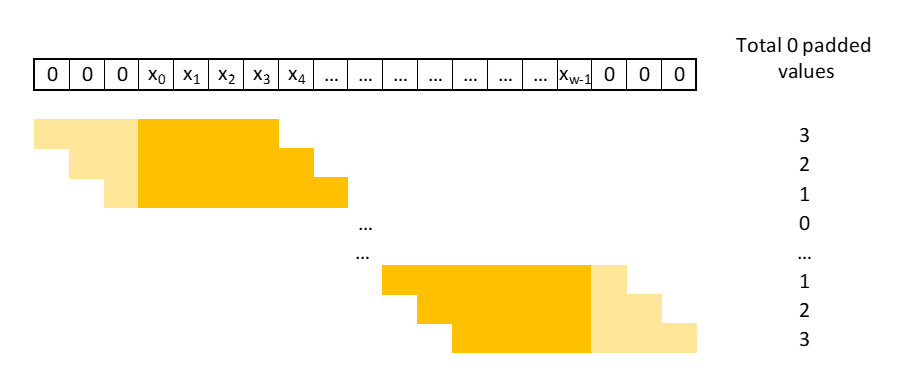
\includegraphics[width=7cm]{img/Conv1D_padding_Nostride}
    \caption{Zero padded elements in a 1D convolution with $k=7 (\bar{k} = 3)$ }
    \label{fig:conv1DNoStride}
\end{figure}

We propose to use Eq.~\ref{eq:ConvApproxLip_app} as a tighter normalization factor\footnote{this factor Eq.~\ref{eq:ConvApproxLip_app} is not a strict upper bound of the lipschitz constant, since particular matrix with high value on the center and low values on borders won't satisfy the inequality~(\ref{eq:CnnMatrix})}.
\begin{equation}
\Lambda=\sqrt{\frac{(k.w-\bar{k}.(\bar{k}+1)).(k.h-\bar{k}.(\bar{k}+1))}{h.w}}
\label{eq:ConvApproxLip_app}
\end{equation}


  

\subsection{Convolution layers with zero padding and stride }
\label{sec:convStride}
Convolution layers are sometimes used with stride (as in Resnet layers~\cite{he_deep_2015}) to reduce the computation cost of these layers\footnote{main drawback with stride is that each point in the input feature map has not the same number of occurrences}. Given a stride $(s,s)$, the output layer size of the layer will be $(wo,ho)$ such as $w=s.wo+rw$ and $h=s.ho+rh$. We also introduce $\alpha=\lceil \frac{k}{s} \rceil$ the maximum number of overlapping stride positions.
As in previous section, we can build a matrix $\bar{X}$ of size $(c.k^2,wo.ho)$, as a duplication of  $\widetilde{X}$. The maximum duplication factor of an element of $\widetilde{X}$ in  $\bar{X}$ is $\Lambda^2=\alpha^2$.

As in section \ref{sec:ConvLayerMatrix}, we can compute a tighter factor using the average duplication factor of input in $X$, by computing the number of non-zero-padded values used in $\bar{X}$. We introduce $\bar{\alpha},\bar{\beta}$ such as $\bar{k}=\bar{\alpha}.s+\bar{\beta}$.

For a 1D convolution  (see Fig.~\ref{fig:conv1DWithStride}), the number of zero values in the first columns of $\bar{X}$ is $(\bar{k},\bar{k}-s,...,\bar{\beta})$. So the number of zero padded values on the left side is $zl=\sum_{t=0}^{\bar{\alpha}}(\bar{k}-t.s)=(\bar{\alpha}+1)\bar{k}-s.\frac{\bar{\alpha}(\bar{\alpha}+1)}{2}=\frac{(\bar{\alpha}+1)(\bar{\alpha}s+2\bar{\beta})}{2}$.

On the right side (last columns), we introduce 
$\gamma_w = argmax\{\gamma=w-1-i.s,  \text{ such as } i>=0  \text{ and }\gamma\leq \bar{k}\}$ i.e. $\gamma_w = w-1-s.\lceil{\frac{w-1-\bar{k}}{s}} \rceil$.  $\gamma_w$ represents the first half-kernel to include the last element of the line. We also introduce $\alpha_w,\beta_w$ such as $\gamma_w = \alpha_w.s+\beta_w$. The number of zero values in the last columns is $(\bar{k}-\gamma_w,\bar{k}-\gamma_w+s,...,\bar{k}-\gamma_w+\alpha_w.s)$, i.e.  $zr_w=\sum_{t=0}^{\alpha_w}(\bar{k}-\gamma_w+t.s)=(\alpha_w+1)(\bar{k}-\gamma_w+\frac{s.\alpha_w}{2})$.
\begin{figure}[htp]
    \centering
    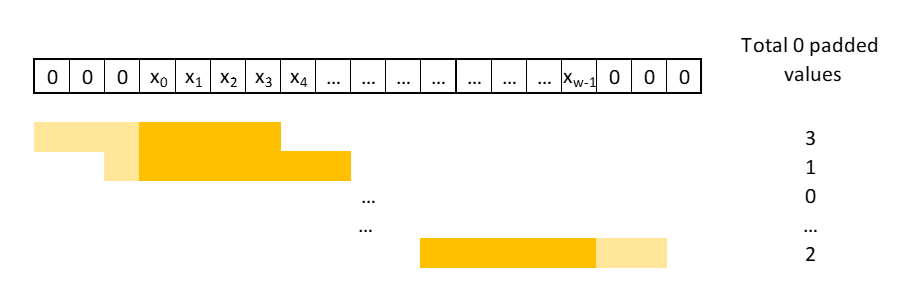
\includegraphics[width=10cm]{img/Conv1D_padding_stride}
    \caption{Zero padded elements in a 1D convolution with stride: $k=7$  $(\bar{k} = 3)$, and $s=2$}
    \label{fig:conv1DWithStride}
\end{figure}

For the matrix $\bar{Y}$ the average duplication factor for a value of the input $X$ is $\frac{(k.wo-zl-zr_w).(k.ho-zl-zr_h)}{h.w}$

We propose to use Eq.~\ref{eq:ConvStrideApproxLip} as a tighter normalization factor\footnote{As in previous section,  this factor is not an upper bound of the lipschitz constant}\footnote{in case of stride $s=1$, we have $\bar{\alpha} = \bar{k}$, $\bar{\beta} = 0$, $\gamma_w= \alpha_w=\bar{k}$ and $\beta_w=0$. So we can retrieve $zl+zr_w=\frac{\bar{k}.(\bar{k}+1)}{2} + \frac{\bar{k}.(\bar{k}+1)}{2}=\bar{k}.(\bar{k}+1)$ }.
\begin{equation}
\Lambda=\sqrt{\frac{(k.wo-zl-zr_w).(k.ho-zl-zr_h)}{h.w}} \label{eq:ConvStrideApproxLip}
\end{equation}


\subsubsection{Pooling layers}
By definition, the max pooling layer is 1-lipschitz, since $||max(X_1)-max(X_2)||\leq ||X_1-X_2||$ \cite{szegedy_intriguing_2013}.

Considering average pooling layer with a averaging size of $po$, and a stride of $s$. Since a mean is equivalent to a convolution with the matrix $\frac{1}{po^2}\mathbbm{1}_{po\times po}$.
The average pooling layer is equivalent to a convolution with stride (sec \ref{sec:convStride}). Introducing $\alpha=\lceil \frac{po}{s} \rceil$, which is $1$ in the common case where $s=po$. So an upper bound of lipschitz constant for  the average pooling layer is  $\Lambda.||W||=\frac{\alpha}{po}$

\iffalse
\vspace{20pt}
Remark: This is coherent with subsampling the input image, which divide the wassertein distance by $\frac{1}{po}$
\fi


\begin{table}[]
    \centering
    \begin{tabular}{|c|c|c|c|}
    \hline
       Layer type  & Parameters &\shortstack{Upper lip  \\constant}   & Thighter Lip estimation \\ \hline
       Dense & & $||W||$ & \\ \hline
       Convolution wo stride& \shortstack{kernel size $(k,k)$\\ $k=2\bar{k}+1$} & $k.||W||$ & $\sqrt{\frac{(k.w-\bar{k}.(\bar{k}+1)).(k.h-\bar{k}.(\bar{k}+1))}{h.w}}.||W||$\\\hline
       Convolution with stride &  \shortstack{kernel size $(k,k)$\\ stride $(s,s)$} & $\lceil \frac{k}{s} \rceil.||W||$ & $\sqrt{\frac{(k.wo-zl-zr_w).(k.ho-zl-zr_h)}{h.w}}.||W||$\\\hline
       MaxPoolig & & $1$ & \\\hline
       AveragePooling & \shortstack{averaging size $po$\\ stride $s$} &$\lceil \frac{po}{s} \rceil.\frac{1}{po}$ & \\ \hline
    \end{tabular}
    \caption{Main }
    \label{tab:wasserstein_estimation}
\end{table}

\subsection{Gradient norm preserving and general architecture}
\label{app:normpreserving}
As proven Sections \ref{sec:khr_properties} and , the optimal function $f^*$ with respect to Equation \ref{eq:reg_OT}, verifies $||\nabla f^* ||=1$ almost surely.
%As pointed out in \ref{wass_prop}, it has been proven in \cite{gulrajani2017improved} that $||\nabla f^* ||=1$ almost everywhere for the optimal function $f^*$ with respect to Equation \ref{kantorovich}.
%Even if the set of continuous function $g$ such as $||\nabla g ||=1 $ (or norm preserving functions) almost everywhere is a subset of 1-Lipschitz functions, it has been shown in \cite{gulrajani2017improved,Anil2019SortingOL} that enforcing this last property, on neural networks, improves the accuracy estimation of the Wasserstein distance.
In \cite{gulrajani2017improved}, the authors propose to add a regularization terms with respect to the average gradient norm with respect to inputs in the loss function. However, the estimation of this value is difficult and a regularization term doesn't guarantee the property. In this paper, we apply the approach described in \cite{pmlr-v97-anil19a}, based on the use of specific activation functions and a normalization process of the weights. 
%In order to have a norm preserving neural networks, activation functions have to be norm preserving. 
Three norm preserving activation functions are proposed:
\begin{itemize}
    \item \textbf{MaxMin} : order the vector by pairs.
    \item \textbf{GroupSort} : order the vector by group of a fixed size.
    \item \textbf{FullSort} : order the vector.
\end{itemize}
These function are vector-wise rather than element-wise. We also propose the activation  \textbf{ConstPReLU}, a PReLU \cite{He_2015} activation function complemented by a constraint such that $|\alpha|\leq 1$ ($\alpha$ the learnt slope). This last function is norm preserving only when $|\alpha|=1$ (linear, or absolute value function), but being computed element wise, it is then more efficient for convolutional layers outputs.

Given a vector $v$ of size $k$ the P-norm pooling is defined in \cite{boureau2010} as follows :
$$
Pool_{P-norm}(v)=\left(\frac{1}{k}\sum_{i=1}^k v_i^p P\right)^{\frac{1}{P}}
$$

Concerning linear functions, a weight matrix $W$ is norm preserving if and only if all the singular values of $W$ are equals to $1$. In \cite{pmlr-v97-anil19a}, the authors propose to use the Björk Orthonormalization algorithm \cite{bjorck71Ortho}. The Björk algorithm compute the closest orthonormal matrix by repeating the following operation :
\begin{equation}
    W_{k+1}=W_k(I+\sum_{i=1}^p(-1)^p \Spvek{-\frac{1}{2};p} Q_k^p)
\end{equation}
where $Q_k=1-W^T_kW_k$ and $W_0=W$.
This algorithm is fully differential, and as for spectral normalization, it is applied during the forward inference, and taken into account for back-propagation.

\section{Experiments : additional results}
\subsection{Networks architecture}
\label{sec:networks_architecture}
 We apply these normalization both to dense and convolutional layers. All the weights are initialized with Björck algorithm with 15 steps. We consider both ReLU and norm preserving activation functions. For convolutional layers, we also apply the lipschitz coefficients correction (Sect.~\ref{sec:ConvLayer1Lip}) and we restrict the norm preserving activation functions to GroupSort-2, and ConstPReLU for efficiency sake\footnote{others regularization layers such as BatchNorm and Dropout are useless and can modify the lipschitz factor}. 
 
 For Two-Moons dataset, the network architecture a MLP with 256-128-64-1 layer sizes. For MNIST 0-8 subset, we use respectively a MLP with 128-64-32-1 layer sizes, or a Convolutional Neural Network, using 3x3 convolution kernels, with C32-C32-P-C64-C64-C64-P-D128-D1 (the same architecture is used with sigmo\"id output.
For Celeb-A male mustache dataset, VGG architecture is used with 3x3 convolution kernels: C16-C16-P-C32-C32-C32-P-C128-C128-C128-P-C256-C256-C256-P-D128-D64-D32-D1. For all experiments Average Pooling have shown better results than maxPooling.
Other experiments were driven with ResNet networks, but leading to the same kind of results.

Lipschitz network were learnt with \Deellip library. After the training step, the weights are replaced by their normalized version %(with additional spectral/Björck steps in order to guarantee the convergence).


\subsection{effect of $\lambda$}
\label{sec:lambda_effect}
The proposed regularized optimal transport for classification is applied on the two digits (0-8) MNIST subset~\cite{Lecun98}, and the CelebA\cite{liu2015faceattributes} male (with-whithout) mustache subset.
Learning is done with the \Deellip library, using the \text{Hinge-KR} loss (Eq.~\ref{eq:reg_OT}), varying the $\lambda$ parameter, using Adam optimizer on 50 epochs, repeated 10 times, and collecting on the test dataset both the Wasserstein distance estimation, and the accuracy.

Fig.~\ref{fig:influence_alpha_param} shows the influence of the hyper-parameter $\lambda$ introduced in eq.~\ref{eq:reg_OT}. %For sake of lisibility, for $\gamma=\inf$, Wasserstein distance estimation  is hidden (lower than 6), and so for $\gamma=0$ and classification accuracy (not 0 centered). 
As expected, the regularization tends to enhance the classification performance, but induce a slight drop on the Wasserstein distance estimation.


%\footnote{{\color{red} expe avec convolution sans le facteur de normalization, ou juste avec le facteur $1/k$? pour valider notre choix}}

%NDLR: j'ai donc enlevé l'influence de la margin.


\begin{figure}
\centering
%%\begin{subfigure}{.5\textwidth}
%%  \centering
%%  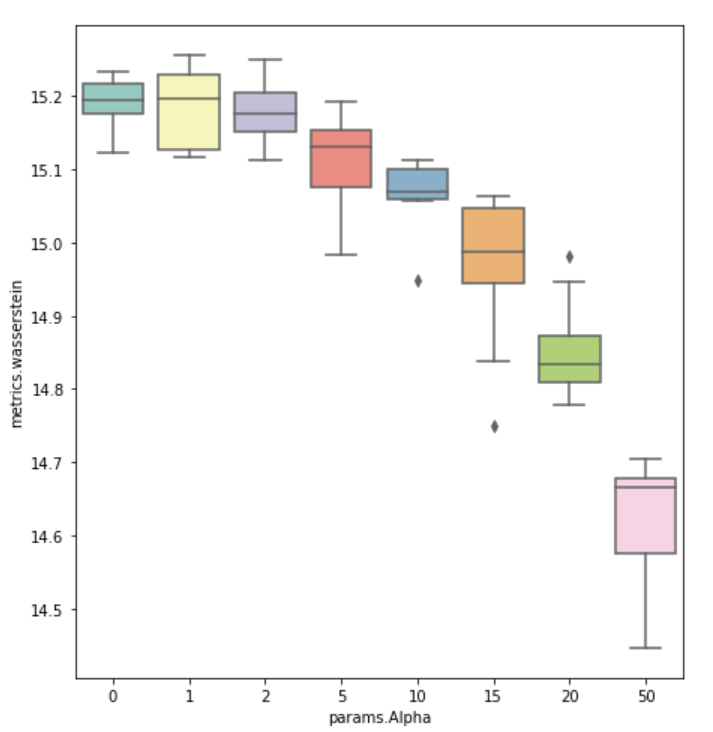
\includegraphics[width=1\linewidth]{img/MNIST08_classifier_param_alpha_wass_metric.png}
%%  \caption{Wasserstein distance estimation}
%%  \label{fig:wass_alpha_param}
%%\end{subfigure}%
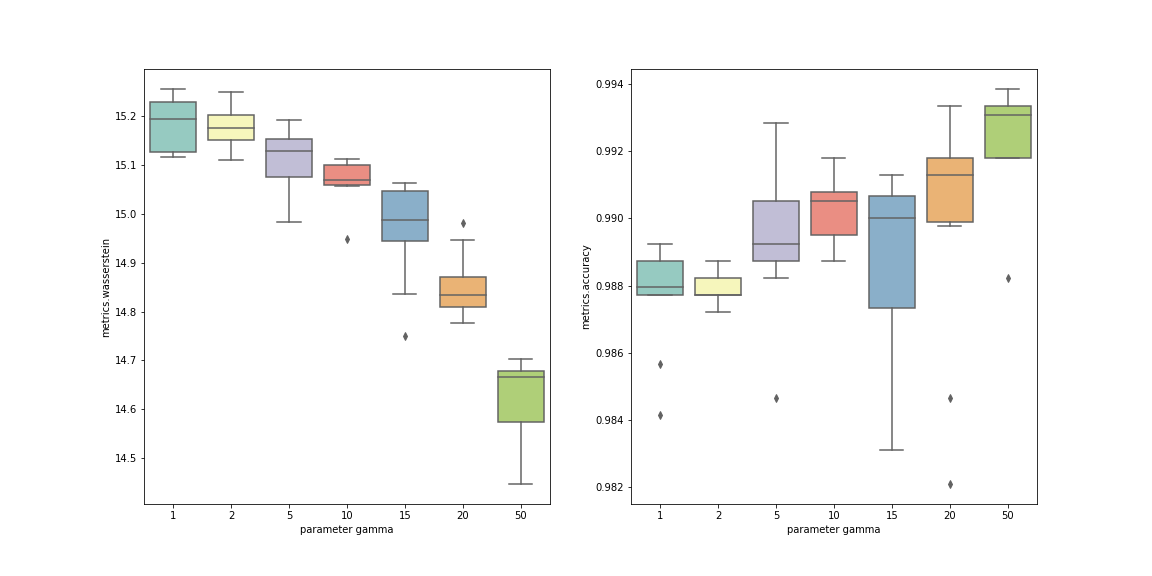
\includegraphics[width=1\linewidth]{img/MNIST08_classifier_param_gamma_wass_accuracy_metric.png}
\label{fig:wass_acc_alpha_param}
\caption{Influence of $\lambda$ hyperparameter on regurarized OT classifier (left: wasserstein distance estimation; right:classification accuracy) with a 1-lipschitz MLP on MNIST 0-8 dataset}
\label{fig:influence_alpha_param}
\end{figure}

\subsection{Approximating Wasserstein distance}
\label{sec:approx_wass_dist}
We first consider the computation of the Wasserstein distance between two distributions using several kind of $Lip_1$ neural networks architectures. The architectures are inspired by \cite{pmlr-v97-anil19a}, but the objective is slightly different, since we are not in the scope of WGAN where the generated distribution aims to decrease this distance. In our scope, the distributions are fixed, and the Wasserstein distance can be computed empirically (\ref{secOptTransp}) as a reference. 

We will compare several kind of $Lip_1$ neural networks, Multi Layer Perceptron and Convolutional Neural Network, with spectral normalization, and Bj\"orck orthonormalization\cite{bjorck71Ortho,pmlr-v97-anil19a}, and activation function ReLU, constrained PReLU (sec. \ref{app:normpreserving}), MaxMin, Groupsort2, FullSort \cite{pmlr-v97-anil19a}. 
Empirical Wasserstein distance is estimated using the POT library\cite{flamary2017pot}, applied on two digits (0-8) MNIST subset\cite{Lecun98}.
%, CelebA\cite{liu2015faceattributes} male (with-whithout) mustache subset.

Learning is done using the \Deellip library with the wasserstein loss (Kantorovich-Rubinstein formulation), and Adam optimizer (initial learning rate $0.01$) on 50 epochs. Each experiment on MNIST dataset are repeated ten times. 

Results presented in table~\ref{tab:wasserstein_estimation} show that the best approximation is obtained using MLP architecture, with Bj\"orck orthonormalization and FullSort activation. It has to be noticed that even for a simple dataset as $MNIST 0-8$, none configuration is able to achieve the empirical Wasserstein distance value. Several possible explanations are possible: it can be due to the representativeness of the chosen $Lip_1$ Neural Network (architecture and activation)  among the $Lip_1$ functions, but it could also be the consequence of an optimization problem. For the former, we use $Lip_1$ layers which gives only an upper bound for the full network lipschitz constant, but has shown in Figure\ref{fig:l2_norm_VGG_wass}, the overall lipschitz factor is close to one. Besides, many experiments (not presented in this paper) have be done on the size and deepness of the Neural networks with roughly the same results. 
For the latter, since the the orthonormalized (Bj\"orck) networks are a subclass of spectral normalization based ones, but results are worse with spectral normalization, optimization issues could be foreseen.  %{\color{red} (Thibaut) cette phrase n'est pas hyper claire: le lien entre les difficultés d'optim et le fait que les réseaux Bj\"ork normalisé soient une ss-classe des réseaux Spectral normalisés n'est pas hyper clair\\
%FRANCK: mon idée était de dire que vu que les Bjorck sont compris dans les spectral norm, l'optimisation devrait permettre d'atteindre les meme resultats, si il n'y arrive pas c'est qu'il y a un pb d'otim. Peut-etre a reformuler}
Experiments done with many type  of optimizers (Adam, SGD, RMSprop,...) lead to the same results, and surprisingly the variance of Wassertein estimations is very low (table~\ref{tab:wasserstein_estimation}). %{\color{red} (FRANCK) to add  in conclusion still a challenge: optimization issue or $Lip_1$ NN representativeness?}

Besides, activation functions choice has also a big influence on the Wasserstein estimation, since choosing ReLU for a MLP leads to a drop of $12\%$ in the estimation.For Convolutional Neural Network, best results for  are obtained with Bj\"orck orthonormalization and constrained PReLU activation, but are worse than MLP. This may be due to the non-invariance to shift and scale of the Wasserstein distance.

\begin{table}[]
    \centering
    \begin{tabular}{|c|c|c|c|c|}
    \hline
       Dataset  & \shortstack{Network \\archi} & Lipschitz type & Activation & Wass estimation \\ \hline
       \multirow{5}{*}{\shortstack{TwoMoons \\($noise=0.05$)}} & [empirical estim.] & N.A. & N.A. & 13.14 \\
        & $MLP_1$  & Bj\"orck (15 it) & FullSort & $\bm{13.13}$  \\
        & $MLP_1$  & Bj\"orck (15 it) & GroupSort2 & 13.11  \\
        & $MLP_1$  & Bj\"orck (15 it) & ReLU & 12.87  \\
        & $MLP_1$  & Spectral norm. & FullSort &  12.88  \\\hline
       \multirow{9}{*}{MNIST 0-8}  & [empirical estim.] & N.A. & N.A. & 19.04 \\
       & $MLP_2$ & Bj\"orck (15 it)  & FullSort &  $\bm{15.20 \pm 0.03}$\\
       & $MLP_2$ & Bj\"orck (15 it)  & GroupSort2 &  $14.60 \pm 0.08$\\
       & $MLP_2$ & Bj\"orck (15 it)  & PReLU &  $13.62 \pm 0.03$\\
       & $MLP_2$ & Bj\"orck (15 it)  & ReLU &  $13.34 \pm 0.07$\\
       & $MLP_2$ & Spectral norm.  & FullSort &  $13.18 \pm 0.40$\\
       & $CNN$ & Bj\"orck (15 it)  & FullSort &  $11.75 \pm 0.29$\\
       & $CNN$ & Bj\"orck (15 it)  & GroupSort2 &  $11.20 \pm 0.05$\\
       & $CNN$ & Bj\"orck (15 it)  & PReLU &  $\bm{12.30 \pm 0.15}$\\
       & $CNN$ & Bj\"orck (15 it)  & ReLU &  $11.11 \pm 0.05$\\
       & $CNN$ & Spectral norm.  & FullSort &  $11.62 \pm 0.23$\\ \hline
    \end{tabular}
    \caption{Wasserstein estimation for various dataset, and various architecture ($MLP_1$: 256,128,64,1; $MLP_2$: 128-64-32-1; CNN : C32-C32-P-C64-C64-C64-P-128-1)}
    \label{tab:wasserstein_estimation2}
\end{table}

%{\color{red} (FRANCK): voir si les figures sont plus intéressantes que les tableaux
%et   comparaison avec clipping, Frobenius?}

\begin{figure}
\centering
\begin{subfigure}{.5\textwidth}
  \centering
  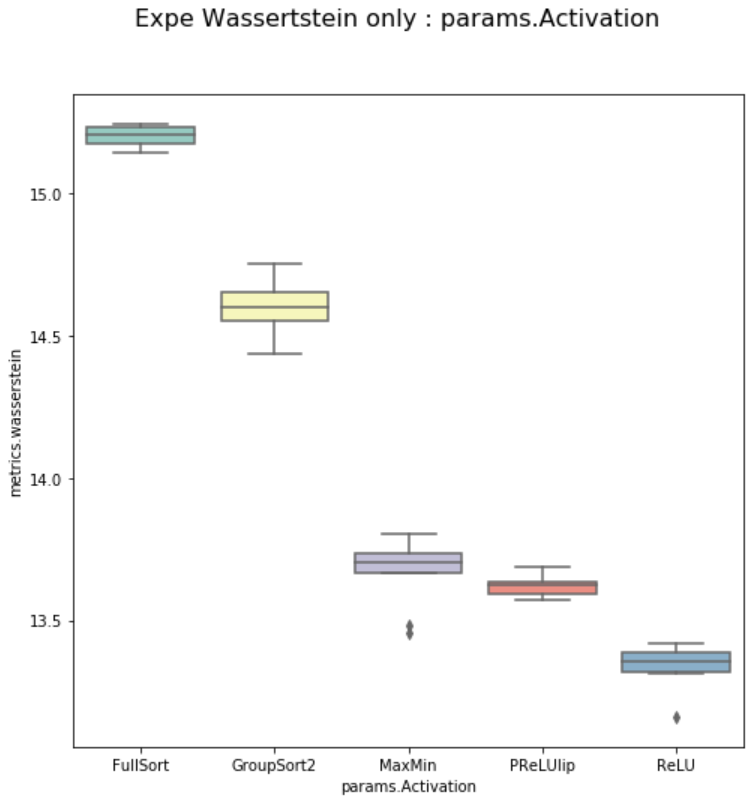
\includegraphics[width=1\linewidth]{img/Wassertein_estimation_MLP_activation_param.png}
  \caption{Variation of activation function}
  \label{fig:sub1}
\end{subfigure}%
\begin{subfigure}{.5\textwidth}
  \centering
  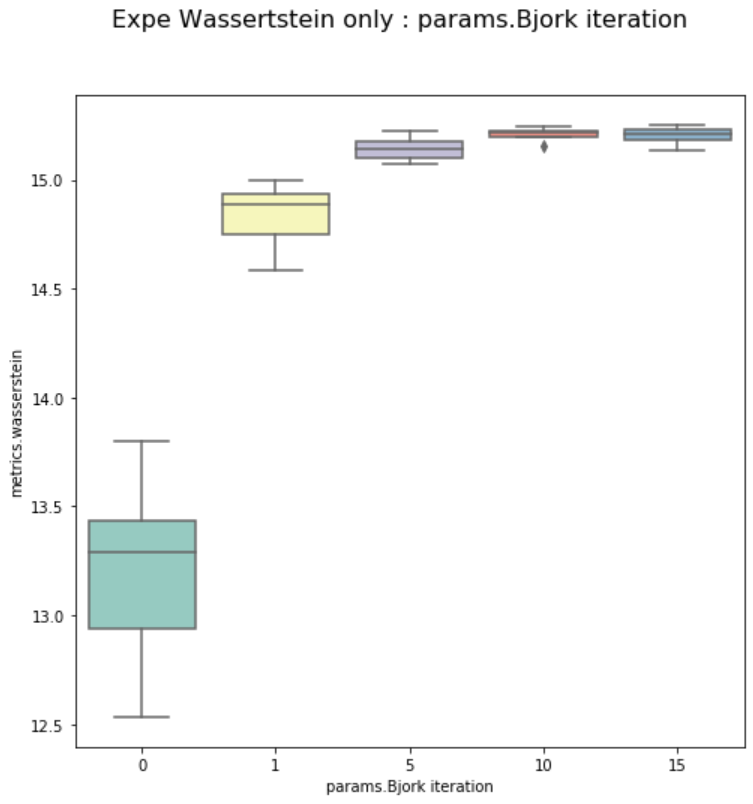
\includegraphics[width=1\linewidth]{img/Wassertein_estimation_MLP_bjorck_param.png}
  \caption{Variation of Bjorck iteration number per batch (0: spectral normalization) using FullSort activation}
  \label{fig:sub2}
\end{subfigure}
\caption{Estimation of Wasserstein distance with a Lipschitz MLP}
\label{fig:wass_estimation_mlp}
\end{figure}

\begin{figure}
\centering
\begin{subfigure}{.5\textwidth}
  \centering
  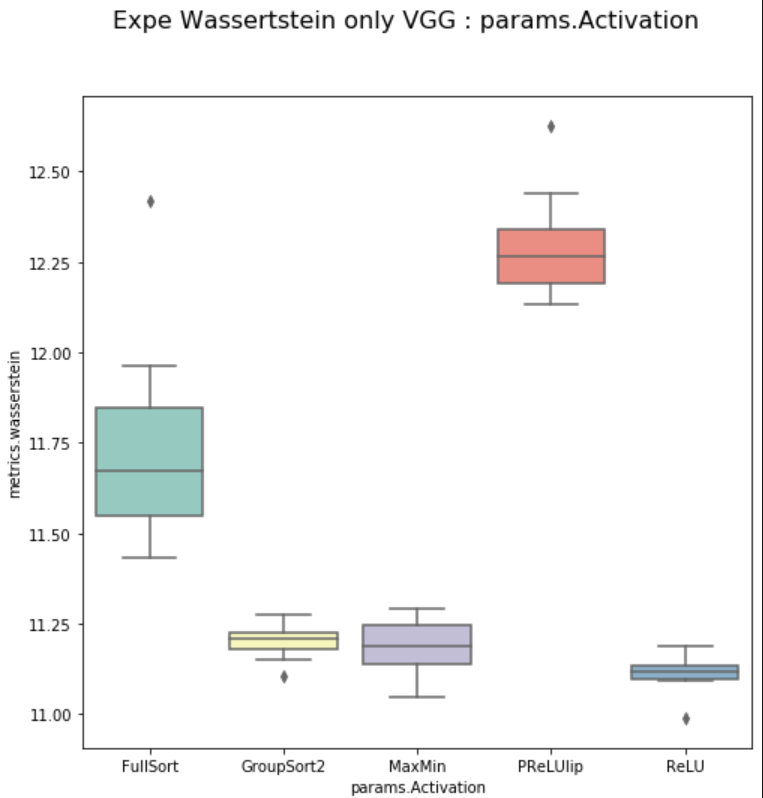
\includegraphics[width=1\linewidth]{img/Wassertein_estimation_VGG_activation_param.png}
  \caption{Variation of activation function}
  \label{fig:act_sub1}
\end{subfigure}%
\begin{subfigure}{.5\textwidth}
  \centering
  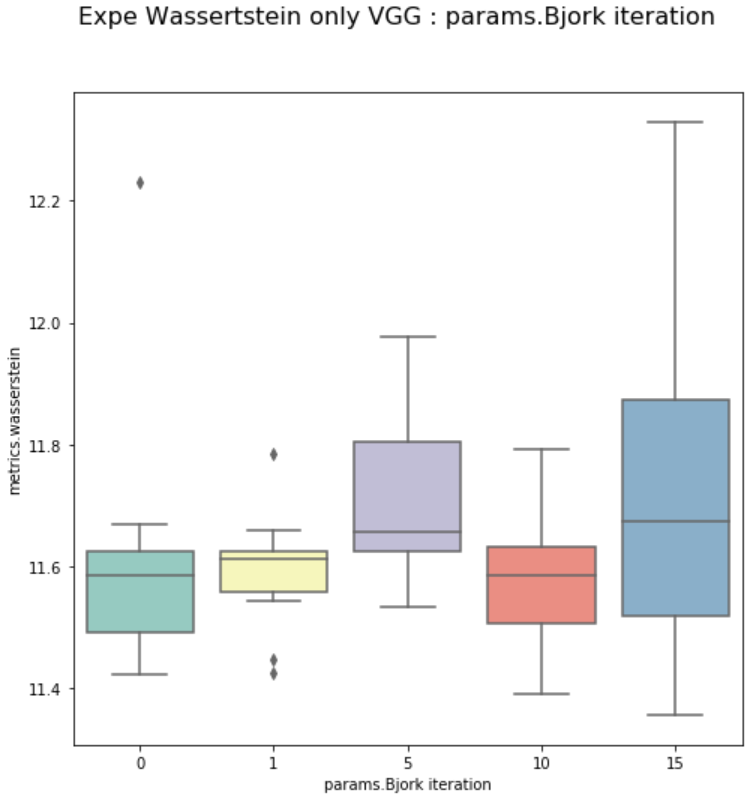
\includegraphics[width=1\linewidth]{img/Wassertein_estimation_VGG_bjorck_param.png}
  \caption{Variation of Bjorck iteration number per batch (0: spectral normalization) using FullSort activation}
  \label{fig:batch_sub2}
\end{subfigure}
\caption{Estimation of Wasserstein distance with a Lipschitz Convolutional Neural Network}
\label{fig:wass_estimation_cnn}
\end{figure}





